\colorbox{white!10!}{
    \begin{minipage}{0.2\textwidth}
       \begin{flushleft}
        \includegraphics[width = 0.6\textwidth]{Эмблема.png}
       \end{flushleft}
    \end{minipage}
    \begin{minipage}[t]{0.7 \textwidth}
        \begin{center}
            {\huge \textsc{Красноярская Летняя Школа. Сезон $7^2 - 2$}}
            \vspace{0.25cm}
            
            { \huge \textbf{ФМТ. Тур 1.}}
        \end{center}
        \vspace{0.05cm}
    \end{minipage}
}

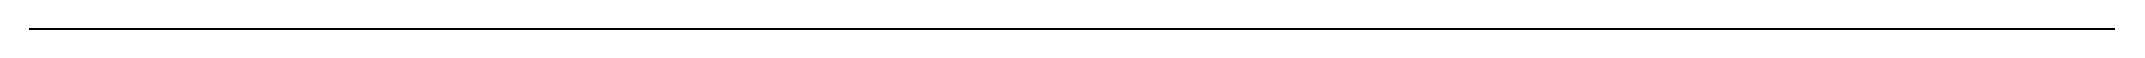
\begin{tikzpicture}
    \draw[thick] (-6.5,0)--(20,0);
\end{tikzpicture}
\begin{enumerate}
    \item Человека, идущего вдоль трамвайных путей, каждые 7 минут обгоняет трамвай. А каждые 5 минут трамвай попадает ему навстречу. Трамваи ходят с одинаковым интервалом. Найдите этот интервал.
    \\
    
    \parbox[b]{.7\textwidth}{%
    \item 
        Определите сопротивление цепи, показанной на схеме. Сопротивление каждого из резисторов $R_0$. Сопротивлением соединительных проводов можно пренебречь. 
    }\hfill\includegraphics[width=.25\textwidth]{pictures/Tur_1.2.png}
\end{enumerate}
   